
\subsection{Lecture de tension des modules}
	\paragraph*{}
	Nous désirons avoir une lecture de tension très précise sur toute la plage d'utilisation des modules. Le circuit doit consommer un minimum de courant, être robuste, modulable et précis. Le circuit doit aussi faciliter la vérification technique.
	
	\subsubsection*{Solution commercial}
	\paragraph*{}
	Il existe sur le marché plusieurs circuit qui s'occupe de lire la tension des modules et de communiquer l'information à un microcontrôleur. Les fonctionnalités et le nombre de modules supportés varient d'un vendeur à l'autre. Les points communs sont : 

	\begin{multicols}{2}
		\begin{itemize}
			\item[$\bullet$] Le circuit peut être alimenté par les modules;
			\item[$\bullet$] Consommation de courant de quelque mA lorsque le circuit prend les mesures et quelque $\mu$A lorsqu'il est en veille;
			\item[$\bullet$] Solution compacte;
			\item[$\bullet$] Lecture précise;
			\item[$\bullet$] Les modules doivent être branchés dans l'ordre;
			\item[$\bullet$] Économique;
			\item[$\bullet$] Fonctionnement bien documenté.
		\end{itemize}
	\end{multicols}

	\paragraph*{}
	Cette solution est réalisable et demande surtout de bien lire et comprendre la documentation. Le LTC6804 de Linear Technology a été retenu pour son nombre de modules maximum, son prix et sa simplicité d'implémentation. Cette solution répond à la majorité des spécifications mais elle n'apporte cependant rien de nouveau au système présentement utilisé et elle ne facilite pas la vérification technique. 
	
	\newpage
	
	\subsubsection*{Isolation des lectures}
	\paragraph*{}
	La vérification technique sera beaucoup plus facile si les différentes lectures de tensions sont isolées. Ce point est décrit dans la section Facilité les manipulations lors des vérifications techniques. 
	
	\paragraph*{}
	L'isolation amène plusieurs avantages :
	
	\begin{itemize}
		\item[$\bullet$] Les modules n'ont plus besoin d'être branchés en ordre, ce qui élimine ce risque d'erreur humaine;
		\item[$\bullet$] Il est possible de débrancher une seule cellule pour venir ensuite la remplacer par une alimentation variable;
		\item[$\bullet$] Le filage dans la batterie peut être mieux organisé et optimisé.
	\end{itemize}

	\paragraph*{}
	Cette solution comporte cependant plusieurs désavantage :
	
	\begin{itemize}
		\item[$\bullet$] Consomme plus de courant (quelque mA par module lors des lectures);
		\item[$\bullet$] Demande plus de composantes;
		\item[$\bullet$] Plus difficile à implémenter;
		\item[$\bullet$] Plus dispendieux.
	\end{itemize}
	
	\paragraph*{}
	Ces différents désavantage ne sont pas majeur dans le contexte d'Éclipse, la consommation de courant reste insignifiante comparé à ce que le moteur et le reste des circuits consomment. Le nombre de composant peut être limité en utilisant la bonne topologie et le prix de la carte peut être plus élevé tant qu'il respecte le budget. 
	
	\subsubsection*{Circuit analogique}
	\paragraph*{}
	Une solution relativement simple et qui ne comporte pas beaucoup de composante est montré à la figure \ref{fig:HCNR201}. Ce circuit très compacte et simple n'est pas assez précis puisque le gain entre les deux photodiodes varie de 5\% pour le HCNR201. Cette erreur fait en sorte que le circuit ne répond pas aux spécifications de +/- 10mV.  
	
	\begin{figure}[H]
		\centering
		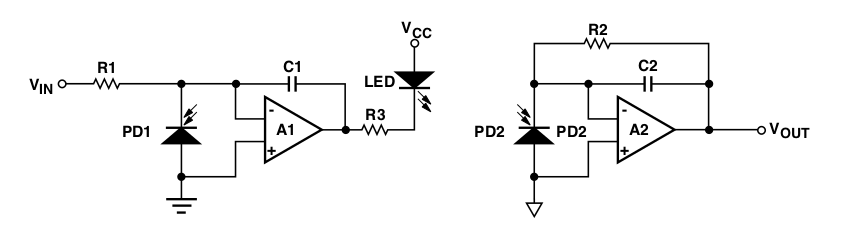
\includegraphics[scale = 0.5]{Images/Analogique.png}
		\caption{Circuit de lecture de tension isolé analogique \cite{HCNR201}}
		\label{fig:HCNR201}
	\end{figure}

	\subsubsection*{Lecture d'un voltage de référence avec un ADC}
	\paragraph*{}	
	
	
	
	
	
	
	
	
	
	